\documentclass[12pt, a4paper]{article}

\usepackage[utf8]{inputenc}
\usepackage[T1]{fontenc}
\usepackage[french]{babel}
\usepackage{geometry}
\usepackage{graphicx}
\usepackage{hyperref}
\usepackage{listings}
\usepackage{xcolor}
\usepackage{tabularx}
\usepackage{float}
\usepackage{enumitem}

\geometry{margin=2.5cm}

\hypersetup{
    colorlinks=true,
    linkcolor=blue!60!black,
    urlcolor=blue!60!black,
    citecolor=blue!60!black,
}

\lstset{
    basicstyle=\ttfamily\small,
    backgroundcolor=\color{gray!8},
    frame=single,
    rulecolor=\color{gray!30},
    breaklines=true,
    captionpos=b,
}

% ---------------------------------------------------------------
% Commande placeholder : affiche un cadre gris en attendant l'image.
% Pour inserer l'image reelle :
%   1. Placer le fichier PNG dans le dossier rapport/
%   2. Remplacer \placeholder{...} par \includegraphics[width=0.85\textwidth]{nom-du-fichier.png}
% ---------------------------------------------------------------
\newcommand{\placeholder}[1]{%
\fbox{\parbox{0.85\textwidth}{\centering\vspace{2.5cm}{\large\color{gray}\textit{#1}}\vspace{2.5cm}}}%
}

% ================================================================
\begin{document}

% --- Page de garde ---
\begin{titlepage}
    \centering
    \vspace*{2cm}
    {\Large \textsc{Architecture des Systèmes d'Information}}\\[0.5cm]
    {\large École d'ingénieurs — Année 2025-2026}\\[2cm]
    \rule{\textwidth}{0.4pt}\\[0.6cm]
    {\Huge \bfseries Projet Microservices\\[0.3cm]
    Application de Location de Logement}\\[0.6cm]
    \rule{\textwidth}{0.4pt}\\[2cm]
    {\large
    % TODO: Mettre les noms du groupe
    \textbf{Groupe :}\\[0.3cm]
    Prénom Nom — Prénom Nom\\
    Prénom Nom — Prénom Nom\\
    }
    \vfill
    {\large Avril 2026}
\end{titlepage}

\tableofcontents
\newpage

% ================================================================
\section{Introduction}

Ce rapport présente la conception et la réalisation d'une application de location de logement basée sur une architecture microservices. Le projet a été réalisé dans le cadre du cours d'Architecture des Systèmes d'Information.

L'objectif principal est de mettre en pratique les concepts vus en cours en construisant une application fonctionnelle où chaque service a une responsabilité claire et peut fonctionner de manière indépendante. Nous avons choisi le cas d'usage d'une plateforme de location (comparable à Airbnb ou Booking) car il se prête bien au découpage en microservices : la gestion des utilisateurs, des logements, des réservations et de la messagerie sont des domaines métier distincts.

Ce document détaille notre réflexion sur le découpage des services, les interactions entre eux, les choix technologiques et la stratégie de déploiement.

% ================================================================
\section{Conception de l'application}

\subsection{Réflexion sur le découpage}

Avant de commencer le développement, nous avons identifié les différents domaines métier de l'application. L'idée était de séparer les responsabilités pour que chaque service gère un périmètre fonctionnel précis. Nous avons retenu le principe suivant : si un domaine peut fonctionner (ou échouer) indépendamment des autres, alors il mérite son propre service.

Par exemple, si le service de messagerie tombe en panne, les utilisateurs doivent pouvoir continuer à naviguer sur les logements et à effectuer des réservations. De même, si le service d'authentification est temporairement indisponible, les logements restent consultables sans connexion. Ce raisonnement nous a conduits à identifier six services backend et deux interfaces frontend.

Nous avons aussi fait le choix de séparer les données : chaque service possède sa propre base de données. Le user-service a sa base PostgreSQL pour les utilisateurs, le property-service a la sienne pour les logements et réservations, et le messaging-service a la sienne pour les messages. Cette séparation empêche un couplage fort entre les services au niveau des données.

\subsection{Vue d'ensemble de l'architecture}

Notre application se compose de six services backend, deux interfaces frontend, trois bases de données PostgreSQL et un service de stockage d'objets (MinIO). Un point d'entrée unique, l'API Gateway, expose l'ensemble de l'application au monde extérieur.

% Schema : fichier mermaid-archi-globale.md
\begin{figure}[H]
\centering
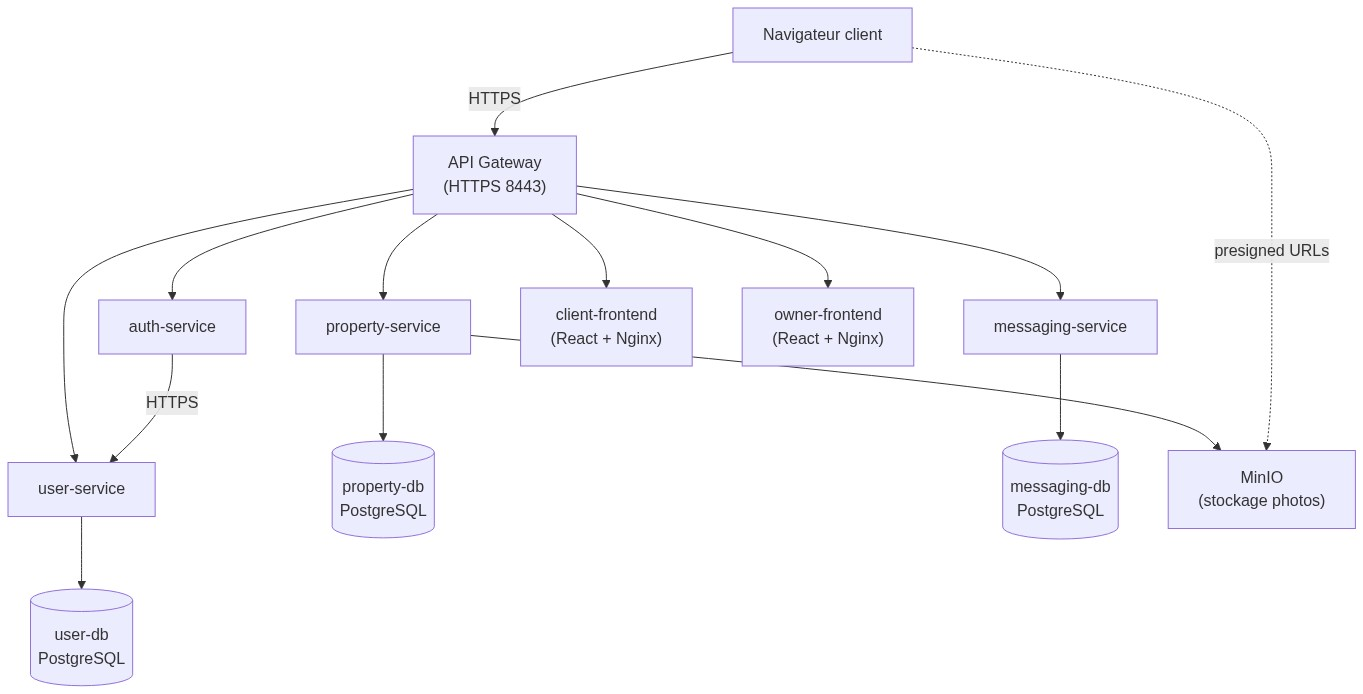
\includegraphics[width=0.85\textwidth]{mermaid-archi-globale.jpg}
\caption{Architecture globale de l'application}
\label{fig:archi}
\end{figure}

\subsection{Description des services}

\subsubsection{API Gateway}

L'API Gateway est le seul point d'entrée exposé à l'extérieur. Tous les appels passent par elle, qu'il s'agisse de requêtes API ou de pages frontend. Son rôle est triple : router les requêtes vers le bon service, valider les tokens JWT pour les routes protégées, et servir les deux interfaces frontend.

Nous avons fait le choix d'un point d'entrée unique car cela simplifie la configuration réseau et la sécurité. Les services internes n'ont pas besoin d'être exposés directement, ce qui réduit la surface d'attaque. Si un service tombe, la gateway retourne une erreur 503 avec un message clair au lieu de laisser le client face à une erreur réseau incompréhensible.

La gateway route les requêtes selon le préfixe de l'URL. Les appels commençant par \texttt{/api/auth/} sont dirigés vers le auth-service, ceux par \texttt{/api/properties/} vers le property-service, etc. Les requêtes vers \texttt{/owner/} servent l'interface propriétaire et toutes les autres servent l'interface locataire.

\subsubsection{Auth-service}

Le auth-service gère l'authentification des utilisateurs. Il expose deux endpoints : l'inscription et la connexion. Lors de la connexion, il vérifie les identifiants en appelant le user-service, puis génère un token JWT si les identifiants sont corrects.

Nous avons séparé l'authentification dans un service dédié car c'est une responsabilité transverse qui ne concerne ni la gestion des logements ni celle des utilisateurs à proprement parler. Le auth-service ne possède pas de base de données propre : il délègue le stockage des données utilisateur au user-service. Ce choix évite la duplication de données.

\subsubsection{User-service}

Le user-service est responsable du stockage et de la gestion des données utilisateur (email, mot de passe hashé, rôle, nom, téléphone). Il expose des endpoints CRUD classiques et sert de source de vérité pour les informations des comptes.

La séparation entre user-service et auth-service permet une chose importante : si le service d'authentification est en panne, les informations utilisateur restent accessibles aux autres services qui en ont besoin. Par exemple, le property-service peut afficher le nom d'un propriétaire sans dépendre du auth-service.

\subsubsection{Property-service}

Le property-service est le service métier principal. Il gère les logements (création, modification, recherche avec filtres) et les réservations (création avec vérification de disponibilité, confirmation, annulation). Il gère aussi les photos des logements via MinIO.

Nous avons regroupé les logements et les réservations dans le même service car ces deux domaines sont fortement couplés : une réservation est toujours liée à un logement, et la recherche de logements prend en compte les réservations existantes pour filtrer par disponibilité. Séparer ces deux aspects aurait engendré beaucoup de communications inter-services pour des opérations simples.

Pour les photos, le property-service ne stocke pas les fichiers. Il génère des URLs pré-signées via MinIO : le navigateur du client envoie les photos directement vers MinIO et les récupère directement depuis MinIO. Le service ne fait que stocker les clés d'objets en base de données. Ce choix allège le service et évite de faire transiter des fichiers volumineux par le backend.

\subsubsection{Messaging-service}

Le messaging-service gère les conversations entre locataires et propriétaires. Une conversation est liée à une réservation confirmée. Chaque message contient l'identifiant de l'expéditeur, son rôle (locataire ou propriétaire), le contenu et un indicateur de lecture.

Nous avons fait le choix d'un service séparé pour la messagerie car c'est une fonctionnalité indépendante du reste. Si ce service tombe en panne, les utilisateurs peuvent toujours chercher des logements, réserver et gérer leurs propriétés. C'est un bon exemple de la résilience que permet l'architecture microservices. La messagerie n'est accessible que pour les réservations confirmées, ce qui lie fonctionnellement les deux services sans les coupler techniquement.

\subsubsection{Interfaces frontend}

Nous avons deux interfaces distinctes : une pour les locataires et une pour les propriétaires. Les locataires accèdent à la recherche de logements, la réservation et la messagerie. Les propriétaires accèdent à la gestion de leurs logements, au suivi des demandes de réservation et à la messagerie.

Les deux frontends sont des applications React servies par Nginx. Elles sont servies par la gateway : l'interface locataire est accessible sur \texttt{/} et l'interface propriétaire sur \texttt{/owner/}. Ce sont deux applications séparées car les besoins sont différents, mais elles partagent le même design system pour la cohérence visuelle.

\subsection{Interactions entre les services}

Les services communiquent entre eux uniquement via des appels HTTP REST en HTTPS. Nous n'avons pas utilisé de message broker (comme RabbitMQ) car les interactions sont synchrones et simples pour notre cas d'usage.

% Schema : fichier mermaid-auth-flow.md
\begin{figure}[H]
\centering
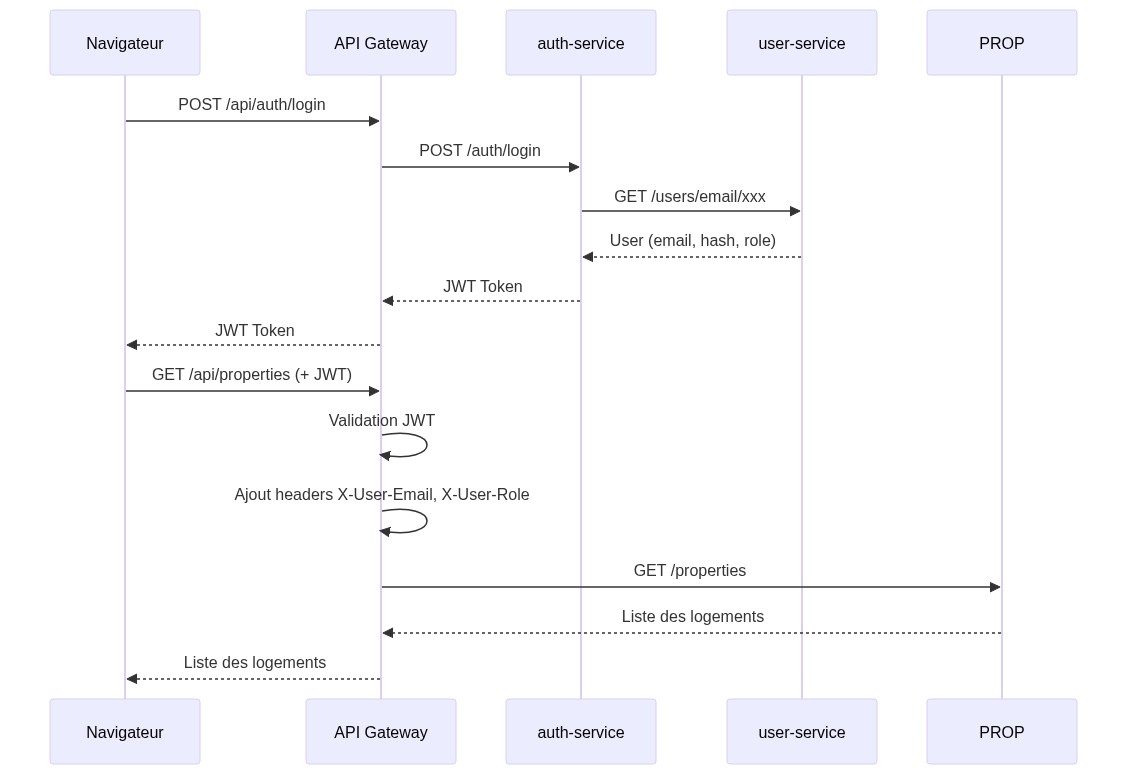
\includegraphics[width=0.85\textwidth]{mermaid-auth-flow.jpg}
\caption{Flux d'authentification et de routage via la gateway}
\label{fig:auth-flow}
\end{figure}

\begin{table}[H]
\centering
\begin{tabularx}{\textwidth}{|l|l|X|}
\hline
\textbf{Appelant} & \textbf{Appelé} & \textbf{Raison} \\
\hline
Navigateur & API Gateway & Toutes les requêtes passent par la gateway \\
\hline
API Gateway & Tous les services & Routage des requêtes selon le préfixe URL \\
\hline
auth-service & user-service & Vérification des identifiants et création de comptes \\
\hline
Navigateur & MinIO & Upload et téléchargement des photos (via URLs pré-signées) \\
\hline
\end{tabularx}
\caption{Interactions entre les services}
\end{table}

Un point important : les services backend ne s'appellent pas directement entre eux (sauf auth-service qui appelle user-service). Le property-service et le messaging-service sont indépendants. La coordination est faite côté client : par exemple, le frontend appelle le property-service pour les détails d'un logement et le messaging-service pour les messages, puis assemble les données.

% Schema : fichier mermaid-reservation-lifecycle.md
\begin{figure}[H]
\centering
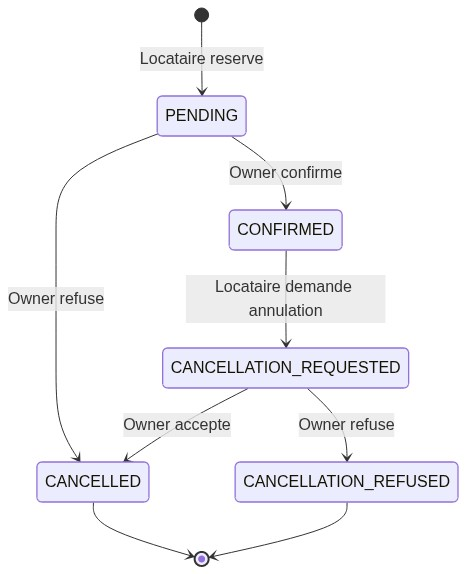
\includegraphics[width=0.75\textwidth]{mermaid-reservation-lifecycle.jpg}
\caption{Cycle de vie d'une réservation}
\label{fig:reservation}
\end{figure}

\subsection{Gestion de la résilience}

Un des objectifs du projet était de montrer que l'application continue de fonctionner même quand certains services sont en panne. Nous avons mis en place plusieurs mécanismes pour cela.

Au niveau de la gateway, un gestionnaire d'erreurs intercepte les erreurs de connexion vers les services internes et retourne une réponse JSON avec un code 503 et le nom du service concerné. Le frontend peut alors afficher un message clair à l'utilisateur.

Au niveau des frontends, chaque page qui appelle un service backend gère le cas où ce service est indisponible. Un composant \texttt{ServiceUnavailable} s'affiche avec un bouton "Réessayer" au lieu de laisser l'utilisateur face à une page blanche.

Nous avons aussi créé une page de statut accessible sur \texttt{/status} qui affiche en temps réel l'état de chaque service avec des pastilles vertes ou rouges. Cette page est utile pour la démonstration.

% TODO: captures d'ecran resilience
\begin{figure}[H]
\centering
\placeholder{Capture : page de statut des services (tous les services actifs)}
% \includegraphics[width=0.85\textwidth]{screenshot-status-page.png}
\caption{Page de statut des services}
\label{fig:status}
\end{figure}

\begin{figure}[H]
\centering
\placeholder{Capture : page d'accueil quand le property-service est arrêté}
% \includegraphics[width=0.85\textwidth]{screenshot-service-down.png}
\caption{Mode dégradé — property-service arrêté}
\label{fig:service-down}
\end{figure}

% ================================================================
\section{Technologies adoptées}

\subsection{Stack technique}

\begin{table}[H]
\centering
\begin{tabularx}{\textwidth}{|l|X|}
\hline
\textbf{Composant} & \textbf{Technologie} \\
\hline
Services backend & Java 17, Spring Boot 3.2.5 \\
\hline
Gateway & Spring Cloud Gateway 2023.0.1 \\
\hline
Authentification & JWT (bibliothèque jjwt 0.12.5) \\
\hline
Bases de données & PostgreSQL 15 \\
\hline
Stockage photos & MinIO (compatible S3) \\
\hline
Frontends & React 18, Vite, React Router \\
\hline
Conteneurisation & Docker, Docker Compose \\
\hline
Communication & HTTPS avec certificats auto-signés \\
\hline
\end{tabularx}
\caption{Stack technique du projet}
\end{table}

Nous avons choisi Java et Spring Boot car c'est la stack vue en cours et la plus utilisée pour les microservices dans l'industrie. Spring Cloud Gateway fournit un mécanisme de routage déclaratif qui nous a permis de configurer toutes les routes dans un fichier YAML sans écrire de logique complexe.

Pour les frontends, nous avons choisi React avec Vite pour sa simplicité de mise en place et sa popularité. Les applications sont construites en images Docker multi-stage (build avec Node.js, puis servies par Nginx).

\subsection{Gestion des interactions entre les services}

Toutes les communications entre services se font en HTTPS avec des certificats auto-signés. Un script \texttt{generate-certs.sh} génère une autorité de certification locale, un certificat serveur, et un keystore PKCS12 partagé entre tous les services Spring Boot. Les services se font confiance via le flag \texttt{useInsecureTrustManager} de la gateway.

Les appels inter-services utilisent RestTemplate (dans le cas du auth-service vers le user-service) avec une configuration SSL qui accepte les certificats auto-signés. Ce n'est pas une pratique de production, mais c'est suffisant pour démontrer le principe du chiffrement des communications.

Les frontends communiquent uniquement avec la gateway via des appels REST en JSON. L'API est préfixée par \texttt{/api/} pour distinguer les routes API des routes frontend.

% Schema : fichier mermaid-minio-flow.md
\begin{figure}[H]
\centering
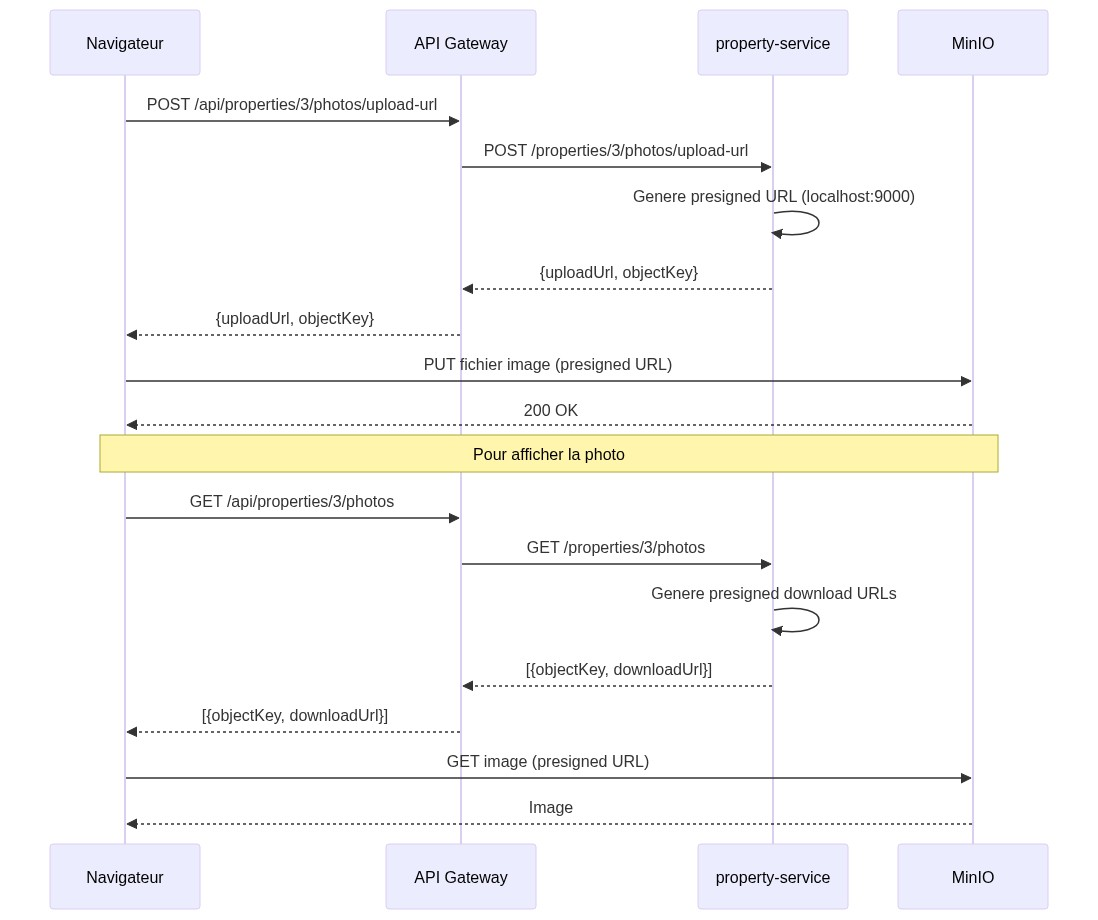
\includegraphics[width=0.85\textwidth]{mermaid-minio-flow.jpg}
\caption{Flux d'upload et de téléchargement des photos via MinIO}
\label{fig:minio}
\end{figure}

\subsection{Gestion de la configuration}

La configuration de chaque service est centralisée dans un fichier \texttt{application.yml}. Les valeurs sensibles ou spécifiques à l'environnement (URL des bases de données, clé secrète JWT, credentials MinIO) sont externalisées via des variables d'environnement, définies dans le \texttt{docker-compose.yml}.

Par exemple, la clé secrète JWT est définie comme \texttt{\$\{JWT\_SECRET:-valeur\_defaut\}} dans la configuration : elle utilise une valeur par défaut pour le développement local mais peut être remplacée en production sans modifier le code.

Nous n'avons pas mis en place de serveur de configuration centralisé (comme Spring Cloud Config) car pour notre nombre de services, la gestion par variables d'environnement est suffisante.

\subsection{Gestion de l'authentification et des habilitations}

L'authentification repose sur des tokens JWT. Lorsqu'un utilisateur se connecte, le auth-service génère un token contenant l'email et le rôle de l'utilisateur (locataire ou propriétaire). Ce token a une durée de validité de 24 heures.

La gateway vérifie le token sur toutes les routes protégées. Les routes publiques (consultation des logements, inscription, connexion) ne nécessitent pas de token. Quand le token est valide, la gateway ajoute les en-têtes \texttt{X-User-Email} et \texttt{X-User-Role} à la requête transmise au service backend. Les services backend peuvent ainsi connaître l'identité de l'utilisateur sans valider le token eux-mêmes.

La clé secrète JWT est partagée entre le auth-service (qui signe les tokens) et la gateway (qui les vérifie). Elle est injectée via une variable d'environnement commune dans le Docker Compose.

\subsection{Gestion du déploiement}

Chaque service est conteneurisé avec Docker. Les Dockerfile suivent le même pattern multi-stage : compilation avec Maven dans une image de build, puis copie du JAR dans une image d'exécution légère (Alpine).

% Schema : fichier mermaid-docker-compose.md
\begin{figure}[H]
\centering
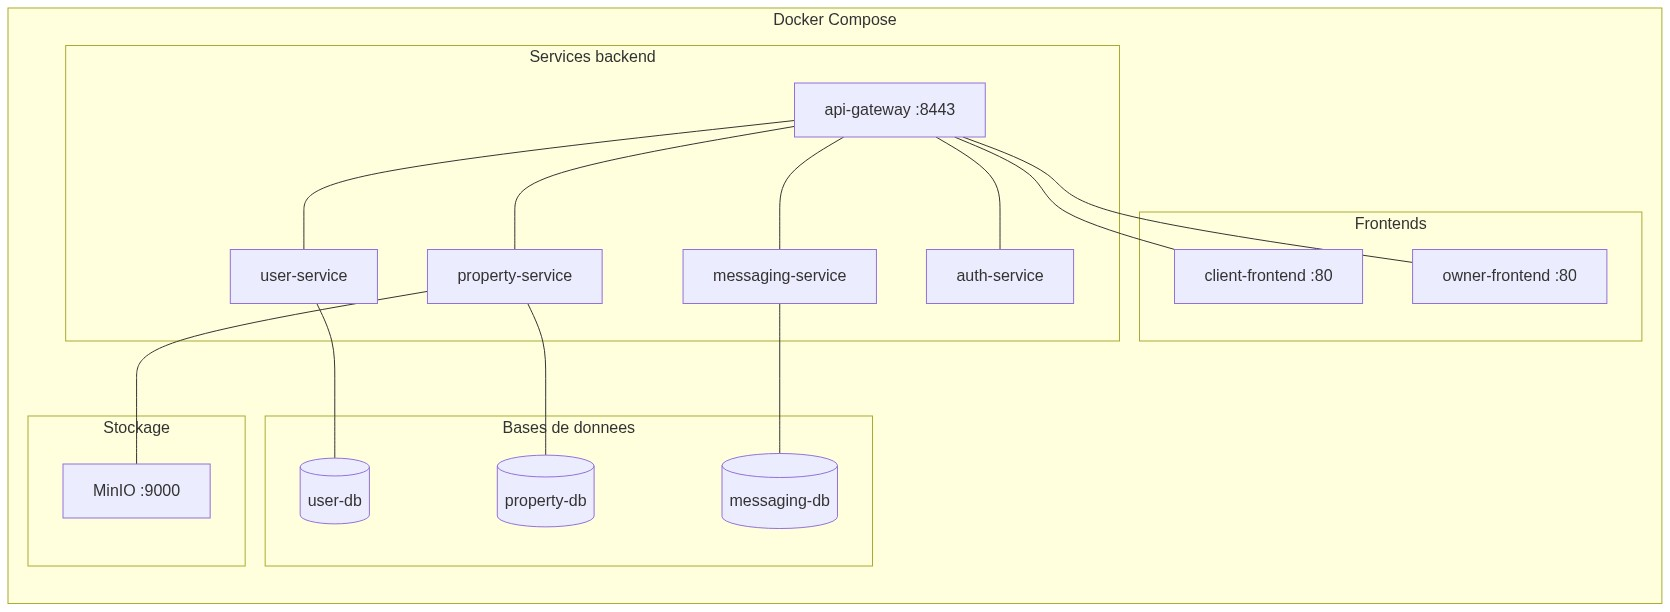
\includegraphics[width=0.85\textwidth]{mermaid-docker-compose.jpg}
\caption{Vue d'ensemble des conteneurs Docker Compose}
\label{fig:docker}
\end{figure}

L'ensemble de l'application est orchestré par Docker Compose. Un \texttt{Makefile} simplifie les commandes courantes :

\begin{table}[H]
\centering
\begin{tabularx}{\textwidth}{|l|X|}
\hline
\texttt{make up} & Génère les certificats, build et lance tous les services \\
\hline
\texttt{make down} & Arrête tous les services \\
\hline
\texttt{make reset-db} & Vide les bases de données et relance (les fixtures se rechargent) \\
\hline
\texttt{make logs} & Affiche les logs de tous les services \\
\hline
\texttt{make clean} & Supprime tout (conteneurs, volumes, certificats) \\
\hline
\end{tabularx}
\caption{Commandes du Makefile}
\end{table}

Le seul prérequis pour lancer l'application est Docker. Les certificats SSL sont générés dans un conteneur Alpine (pas besoin d'OpenSSL sur la machine hôte), les services Java sont compilés dans des conteneurs Maven, et les frontends sont construits dans des conteneurs Node.js.

Des données de démonstration (comptes utilisateurs, logements, réservations, messages) sont automatiquement insérées au démarrage de chaque service via des \texttt{CommandLineRunner} Spring Boot.

\subsection{Gestion des erreurs et logging}

Chaque service backend utilise un \texttt{@RestControllerAdvice} qui intercepte toutes les exceptions et retourne un format d'erreur JSON uniforme :

\begin{lstlisting}
{
  "status": 404,
  "error": "Not Found",
  "message": "Logement non trouve : 42",
  "service": "property-service",
  "timestamp": "2026-04-07T12:00:00"
}
\end{lstlisting}

Ce format est le même pour tous les services, ce qui permet aux frontends de traiter les erreurs de manière homogène. Les exceptions custom (\texttt{EntityNotFoundException}, \texttt{ConflictException}) sont mappées vers les codes HTTP appropriés (404, 409).

Le logging utilise SLF4J (inclus dans Spring Boot). Chaque requête entrante et chaque erreur sont loggées avec le nom du service pour faciliter le diagnostic dans les logs Docker Compose.

% ================================================================
\section{Fonctionnalités réalisées}

\subsection{Côté locataire}

L'interface locataire permet de rechercher des logements par ville, dates de disponibilité, type et prix maximum. Les résultats s'affichent sous forme de cartes avec la photo du logement. La page de détail permet de consulter les informations, les photos et de réserver en sélectionnant des dates. Les dates déjà réservées sont grisées dans le calendrier.

Le locataire peut suivre ses réservations (en attente, confirmée, annulée), demander une annulation, et communiquer avec le propriétaire via la messagerie une fois la réservation confirmée.

% TODO: captures d'ecran locataire
\begin{figure}[H]
\centering
\placeholder{Capture : page d'accueil avec recherche de logements}
% \includegraphics[width=0.85\textwidth]{screenshot-homepage.png}
\caption{Page d'accueil — recherche de logements}
\label{fig:homepage}
\end{figure}

\begin{figure}[H]
\centering
\placeholder{Capture : page de détail d'un logement avec calendrier}
% \includegraphics[width=0.85\textwidth]{screenshot-property-detail.png}
\caption{Page de détail d'un logement}
\label{fig:detail}
\end{figure}

\begin{figure}[H]
\centering
\placeholder{Capture : page "Mes réservations" côté locataire}
% \includegraphics[width=0.85\textwidth]{screenshot-reservations-tenant.png}
\caption{Mes réservations — côté locataire}
\label{fig:reservations-tenant}
\end{figure}

\begin{figure}[H]
\centering
\placeholder{Capture : messagerie côté locataire}
% \includegraphics[width=0.85\textwidth]{screenshot-messagerie-tenant.png}
\caption{Messagerie — côté locataire}
\label{fig:msg-tenant}
\end{figure}

\subsection{Côté propriétaire}

L'interface propriétaire donne accès à un tableau de bord avec la liste des logements. Le propriétaire peut ajouter, modifier et supprimer des logements, gérer les photos, et consulter les demandes de réservation. Il peut confirmer ou refuser une réservation, accepter ou refuser une demande d'annulation, et communiquer avec les locataires.

Un système de notifications indique le nombre de réservations en attente et de messages non lus directement dans la barre de navigation.

% TODO: captures d'ecran proprietaire
\begin{figure}[H]
\centering
\placeholder{Capture : tableau de bord propriétaire}
% \includegraphics[width=0.85\textwidth]{screenshot-dashboard-owner.png}
\caption{Tableau de bord — côté propriétaire}
\label{fig:dashboard}
\end{figure}

\begin{figure}[H]
\centering
\placeholder{Capture : page des réservations avec notifications}
% \includegraphics[width=0.85\textwidth]{screenshot-reservations-owner.png}
\caption{Réservations avec notifications — côté propriétaire}
\label{fig:reservations-owner}
\end{figure}

\begin{figure}[H]
\centering
\placeholder{Capture : messagerie côté propriétaire}
% \includegraphics[width=0.85\textwidth]{screenshot-messagerie-owner.png}
\caption{Messagerie — côté propriétaire}
\label{fig:msg-owner}
\end{figure}

\subsection{Résilience}

Quand un service backend est arrêté, l'application continue de fonctionner en mode dégradé. Les pages affichent un composant "Service temporairement indisponible" avec un bouton pour réessayer. Une page de statut montre l'état de chaque service en temps réel.

% TODO: capture resilience
\begin{figure}[H]
\centering
\placeholder{Capture : démonstration de résilience (un service coupé)}
% \includegraphics[width=0.85\textwidth]{screenshot-resilience-demo.png}
\caption{Mode dégradé — démonstration de résilience}
\label{fig:resilience}
\end{figure}

% ================================================================
\section{Conclusion}

Ce projet nous a permis de mettre en pratique les concepts d'architecture microservices dans un cas concret. Le découpage en services indépendants, chacun avec sa propre base de données et sa propre responsabilité, nous a montré les avantages de cette approche : déploiement indépendant, résilience aux pannes, et séparation claire des responsabilités.

Nous avons aussi constaté les défis : la gestion de la communication HTTPS entre services, la propagation de l'authentification via JWT, et la complexité de l'infrastructure Docker Compose avec de nombreux conteneurs. Le projet final comporte six services backend, deux frontends, trois bases de données, un service de stockage et une gateway, soit plus de douze conteneurs Docker.

Parmi les améliorations possibles, nous pourrions ajouter un service de configuration centralisé (Spring Cloud Config), un service discovery (Eureka), du load balancing avec plusieurs instances de chaque service, ou un message broker pour les communications asynchrones. Ces ajouts seraient pertinents dans un contexte de production mais dépassent le cadre de ce projet éducatif.

\end{document}
